\documentclass{standalone}
\usepackage{tikz}
\usepackage{verbatim}
\begin{document}
\pagestyle{empty}
  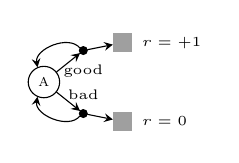
\begin{tikzpicture}
    \node[draw,circle,scale=2/3] (a) at (+0, 0) {\scriptsize A};
    \node[draw,circle, fill, scale=0.3,label=below:{\tiny good}] (g) at (+0.5, 0.4) {};
    \node[draw,circle, fill, scale=0.3,label=above:{\tiny bad}] (b) at (+0.5, -0.4) {};
    \node[draw,rectangle,fill,gray!75,label=right:{\tiny $r = +1$}] (p) at (+1, 0.5) {};
    \node[draw,rectangle,fill,gray!75,label=right:{\tiny $r = 0$}] (n) at (+1, -0.5) {};
    \draw[-stealth]  (a) -- (g);
    \draw[-stealth]  (a) -- (b);
    \draw[-stealth]  (g) -- (p);
    \draw[-stealth]  (b) -- (n);
    \path[-stealth] (b) edge[bend left=75] (a);
    \path[-stealth] (g) edge[bend right=75] (a);
  \end{tikzpicture}
\end{document}